
%(BEGIN_QUESTION)
% Copyright 2012, Tony R. Kuphaldt, released under the Creative Commons Attribution License (v 1.0)
% This means you may do almost anything with this work of mine, so long as you give me proper credit

A 120 pound weight is dragged along a level surface with a steady pull of 25 pounds for 10 feet.  How much work is done (express your answer in both English and metric units of work)?

$$\includegraphics[width=15.5cm]{i02589x01.eps}$$

\underbar{file i02589}
%(END_QUESTION)





%(BEGIN_ANSWER)

In this problem, the figure of 120 lb is of no consequence to our calculations.  What matters is the 25 pound force {\it in the direction of the weight's displacement}.  Since there is no displacement (motion) in the direction of the 120 pound force (straight down), there is no work performed by that force.


$$W = Fx \cos \theta$$

$$W = (25 \hbox{ lb})(10 \hbox{ ft})(\cos 0^o)$$

$$W = 250 \hbox{ ft-lb}$$

We may convert units directly from ft-lb to J in one step, forming a ``unity fraction'' with the equivalence :

$$\left(250 \hbox{ ft-lb} \over 1 \right) \left(1055.06 \hbox{ J} \over 778.169 \hbox{ ft-lb} \right) = 338.96 \hbox{ J}$$

%(END_ANSWER)





%(BEGIN_NOTES)


%INDEX% Physics, energy, work, power

%(END_NOTES)


